\chapter{Referencial Teórico}
Neste Capítulo, serão abordados alguns conceitos e técnicas necessárias para
compreender o trabalho proposto, que é 
gerar malha e mapa de altura com tamanho pseudo-infinitos, de maneira procedural
e não assistida, suportando mais de um bioma.
Se entende por técnica não assistida quando não é necessário intervenção humana nos 
terrenos gerados pelo algoritmo \cite{gabrielle2016canion}.

\section{Biomas}
Neste trabalho o conceito de bioma é padrões de relevo, já que o resultado do trabalho
é mapas de altura, então a única característica que é relevante
são as altitudes do solo e seus padrões, descartando dados como tipo da
vegetação e sua distribuição, umidade e entre outros. Então no restante 
do trabalho, quando for usado os termos "característica do bioma", o mesmo vai
se referir a alguma característica de altitude do bioma. Cor é uma característica 
para ajudar na percepção de biomas distintos em um mapa.

Para fins de restringir o escopo do projeto vamos agrupar os biomas por padrões
de relevo e não por fauna e flora como feito nos conceitos mais conhecidos.

Como este trabalho é voltado para a área de jogos, dentro da comunidade de jogadores
é bem aceito usar o termo bioma de forma mais genérica. O jogo Minecraft usa o
termo e entre seus biomas se encontra \textit{Extreme Hills} e \textit{Plains}.

Normalmente jogos tem um padrão de arte, os biomas que neles são mostrados não 
precisam ser realistas e nem respeitar a natureza real ou as regras da física. Aqui será 
abordado a implementação de uma técnica que consiste em separar regiões de biomas, e criar
um terreno aplicável para jogos com múltiplos biomas.

\section{Representação das Regiões}
%Um bioma vai pertencer a um conjunto de regiões, na imagem \ref{fig:squadStripBiomes}
%que usa uma malha de quadrados, onde os segmentos de retas vermelhas são fronteiras entre
%biomas.
A maneira de separar regiões de biomas é com áreas quadradas, cada uma delas com
tamanho $b^{2}$, cada região tem um identificador $(dxs, dzs)$, esse identificador
será usado como entrada em uma função de ruído, O valor retornado deste ruído vai 
determinar o bioma da região em questão. Na figura \ref{fig:squadStripBiomes} temos
um exemplo com várias regiões, algumas dessas regiões fazendo fronteira entre biomas, 
nela é visível 3 biomas distintos.

\begin{figure}[H]
    \centering
    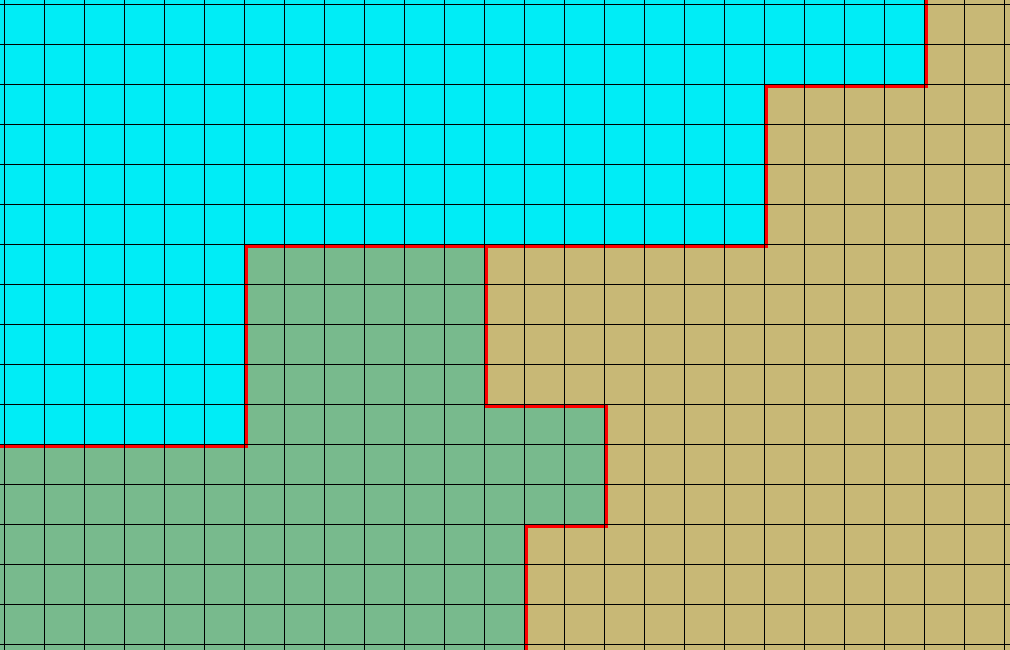
\includegraphics[width=0.7\textwidth]{figuras/squadStripBiomes.png}
    \caption{Malha de quadrados com divisão de biomas}
    \label{fig:squadStripBiomes}
\end{figure}
\section{Malha de terrenos}
\subsection{Malhas de quadrado}
Este modelo é apresentado na figura \ref{fig:squadStripBiomes}, nele cada
quadrado é uma região. Os vértices armazenados se encontram nos quatro cantos
do quadrado, então um vértice é comum a quatro quadrados, cada um deles
compartilhando o vértice com os quadrados adjacentes, as arestas entre vértices
vizinhos são uma fronteira entre regiões, e tem a possibilidade desta aresta ser
também uma fronteira entre biomas.

Devido ao padrão podemos perceber que não há necessidade de armazenar arestas
em memória, já que a mesma só vai existir entre vértices vizinhos, o vértice
$v_{i, j}$ tem como vizinhos o conjunto $\{v_{i+1, j}, v_{i-1, j}, v_{i, j+1}, v_{i, j-1}\}$.
\subsection{Malha triangular}
Usando a mesma base de vértice da malha de quadrados, agora temos uma aresta
adicional, uma diagonal em cada quadrado do modelo anterior, dividindo a região
em duas, cada triangulo sendo uma região, como podemos ver na figura \ref{fig:vbo}.
Agora além do conjunto de arestas do modelo anterior, o vértice $v_{i, j}$ também tem
aresta para os vértices $\{v_{i+1, j+1}, v_{i-1, j-1}\}$.

\begin{figure}[H]
    \centering
    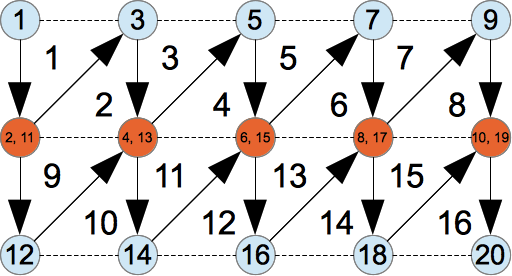
\includegraphics[width=0.5\textwidth]{figuras/vbo.png}
    \caption{Malhas de triângulos, retirado de \cite{androidtrianglestrip}}
    \label{fig:vbo}
\end{figure}

O terreno precisa ser formado por polígonos, para que seja possível renderizar pedaços de planos.
Se a quantidade de vértices por polígono for maior que $3$, então tem pelo menos um ponto com altura sendo uma 
variável não livre. Mas neste trabalho a altura de todos os vértices precisa ser varável livre, logo o terreno será representado por uma malha de triângulos.
%\subsection{Diagrama de Voronoi}
%Um diagrama de Voronoi é uma partição no plano para separar regiões, recebendo
%como entrada um conjunto de pontos chamados de \textit{sites}, o algoritmo
%separa as regiões de cada \textit{site} deixando a fronteira equidistante entre eles
%\cite{fortune1987sweepline}.
%
%Como está implementação vai ser não assistida estes sites precisam ser colocados
%aleatoriamente e proceduralmente, para não ocorrer aglomerações de site, já
%que existe a possibilidade de acontecer na geração de \textit{sites} aleatórios,
%será usado o algoritmo de Lloyd's para relaxar os sites, o conjunto dessas
%técnicas já foi usado por \cite{patel2010polygonal}, para gerar malha de regiões,
%segue uma imagem de seu diagrama na figura \ref{fig:voronoi-2-lloyd}, este diagrama
%foi usado para alcançar o resultado já mostrado na ilustração \ref{fig:voronoi-map-goal-distorted}.
%\begin{figure}[H]
%    \centering
%    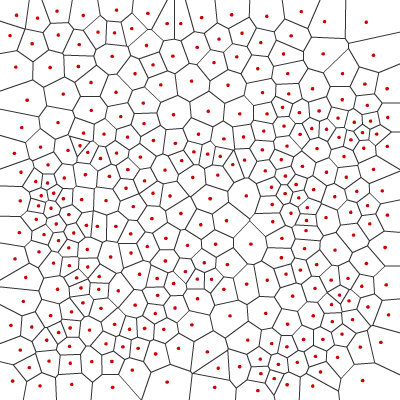
\includegraphics[width=0.5\textwidth]{figuras/voronoi-2-lloyd.png}
%    \caption{Diagrama de Voronoi com algoritmo de Lloyd's aplicado, por \cite{patel2010polygonal}}
%    \label{fig:voronoi-2-lloyd}
%\end{figure}

\section{Ruído de Perlin}
Bons geradores de números aleatórios geram números onde não existe relação entre
eles, porem se montado um gráfico com eles, o resultado não teria um aspecto
orgânico, então para o terreno ter um relevo mais parecido com o encontrado na 
natureza é usado uma função de ruído \cite{shiffman2012nature}, está comparação
pode ser feita com a imagem \ref{fig:randomAndNoise}. 
A função de ruído usa interpolação de pontos aleatórios para determinar seu resultado.
Por exemplo podemos determinar a altura$(y)$ em um gráfico, usando $(x)$ como 
parâmetro, tendo $y = Noise(x)$, uma possível representação seria a parte da esquerda na
figura \ref{fig:randomAndNoise}, tendo o ($x$) na horizontal ($y$) na vertical.
\begin{figure}[H]
    \centering
    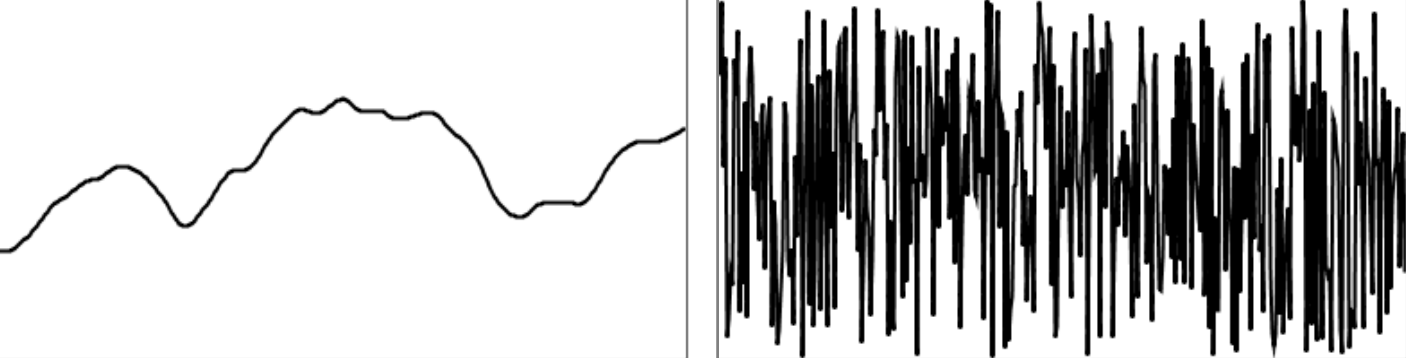
\includegraphics[width=0.7\textwidth]{figuras/randomAndNoise.png}
    \caption{Na esquerda uma função de ruído, na direita pontos aleatórios de uma função \textit{rand}. Por \cite{shiffman2012nature}}
    \label{fig:randomAndNoise}
\end{figure}

Uma função de ruído recebe como parâmetro as coordenadas em um espaço de $n$ dimensões e
retorna um valor entre $-1$ e $1$ para tal posição\cite{shiffman2012nature}.

Na figura \ref{fig:randomAndNoise} vimos o ruído unidimensional, o ruído
tem a complexidade $O(2^n)$, sendo $n$ a quantidade de dimensões \cite{zucker2001perlin}.
Este mesmo ruído unidimensional pode ser usado nas fronteiras entre biomas, dando
um aspecto mais natural á fronteiras, da mesma maneira que foi usado nas bordas
das ilhas no trabalho de \cite{patel2010polygonal}. Contudo, para gerar altura
em um cenário tridimensional precisamos usar o ruído bidimensional. Existem
implementações do ruído em placas gráficas que calculam a função de ruído para 
$\{1, 2, 3\}$ dimensões em único ciclo \cite{perlin2002improving}.

No ruído unidimensional a resposta é uma interpolação entre os seus vizinhos, que
neste caso são apenas $2$. Caso o parâmetro do ruído for $x_{i}$, o mesmo só tem 
como vizinhos, $x_{i+1}$ e $x_{i-1}$, quando a dimensão aumenta e por conta disso
os parâmetros também, a quantidade de vizinhos também aumenta \cite{shiffman2012nature}, 
como o mesmo exemplifica na ilustração \ref{fig:1dto2dnoise}.
\begin{figure}[H]
    \centering
    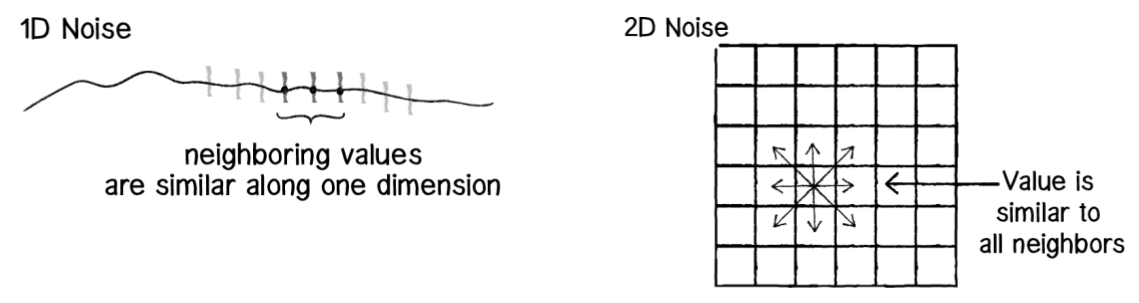
\includegraphics[width=0.7\textwidth]{figuras/1dto2dnoise.png}
    \caption{Vizinhas para função de ruído, $1d$ para $2d$. Por \cite{shiffman2012nature}}
    \label{fig:1dto2dnoise}
\end{figure}

O \textit{ruído de Perlin} usa a função ruído várias vezes, cada uma é chamada
de oitava. Oitava usa amplitude e frequência diferente, a primeira oitava é gerada com uma
amplitude alta e frequência baixa, a próxima oitava tem a metade da amplitude e 
o dobro da frequência. Cada oitava tem a metade da amplitude e o dobro da frequência da oitava anterior.
O ruído de Perlin é a soma de todas as oitavas computadas,
adaptado de Hugo Elias \cite{carli2012canion} gerou as imagens
\ref{fig:perlin1d} e \ref{fig:perlin2d} do ruído de Perlin em uma e duas
dimensões respectivamente. Na imagem \ref{fig:perlin1d} pode ser visto seis oitavas.
\begin{figure}[H]
    \centering
    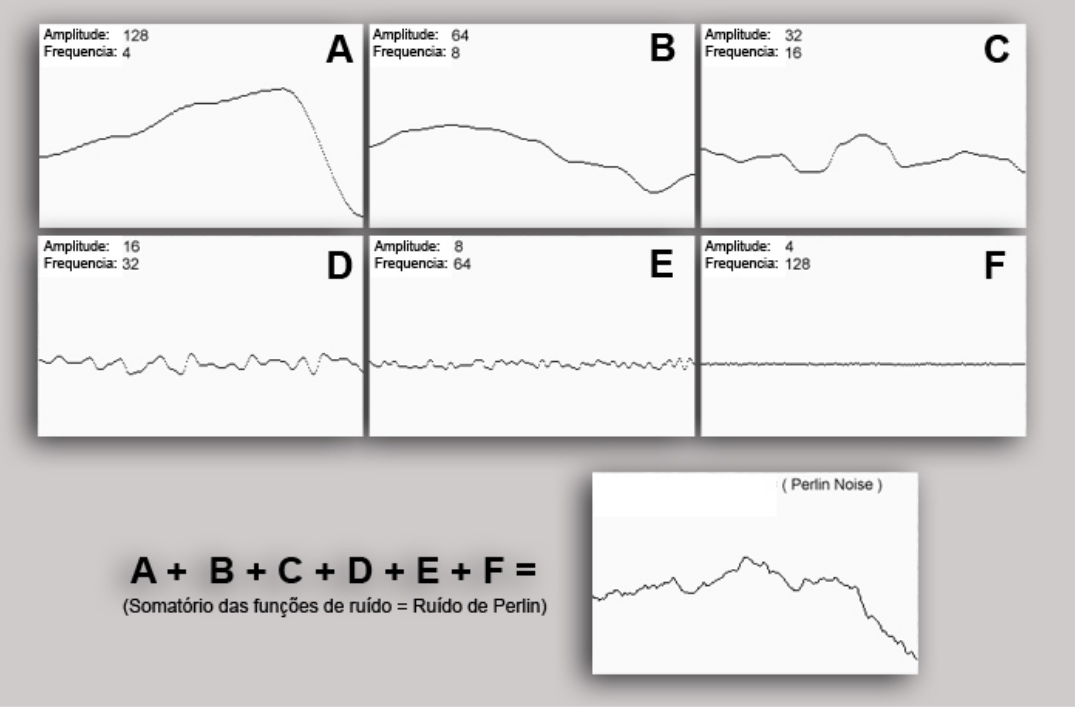
\includegraphics[width=0.7\textwidth]{figuras/perlin1d.png}
    \caption{Gerando ruído de Perlin para uma dimensão}
    \label{fig:perlin1d}
\end{figure}
\begin{figure}[H]
    \centering
    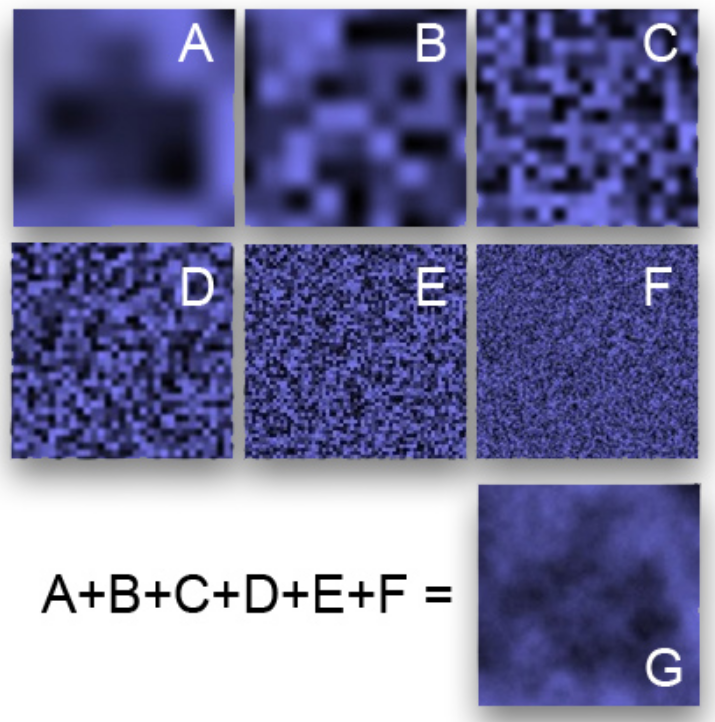
\includegraphics[width=0.6\textwidth]{figuras/perlin2d.png}
    \caption{Gerando ruído de Perlin para duas dimensões}Interpolação
    \label{fig:perlin2d}
\end{figure}

\section{Mapas de Altura}
Mapas de altura é uma maneira de representar altitudes de um terreno. Mapas de altura são imagens
onde os pontos mais claros representam pontos mais elevados e os escuros regiões mais baixas.
A imagem \ref{fig:perlin2d} já traz exemplos de mapas de altura.

Um mapa de altura pode ser usado para ser renderizado em diferentes perspectivas,
ou para usar processos que geram imagens de luz e sombra, ilustrados na figura \ref{fig:hmap} de \cite{dachsbacher2006interactive}.
\begin{figure}[H]
    \centering
    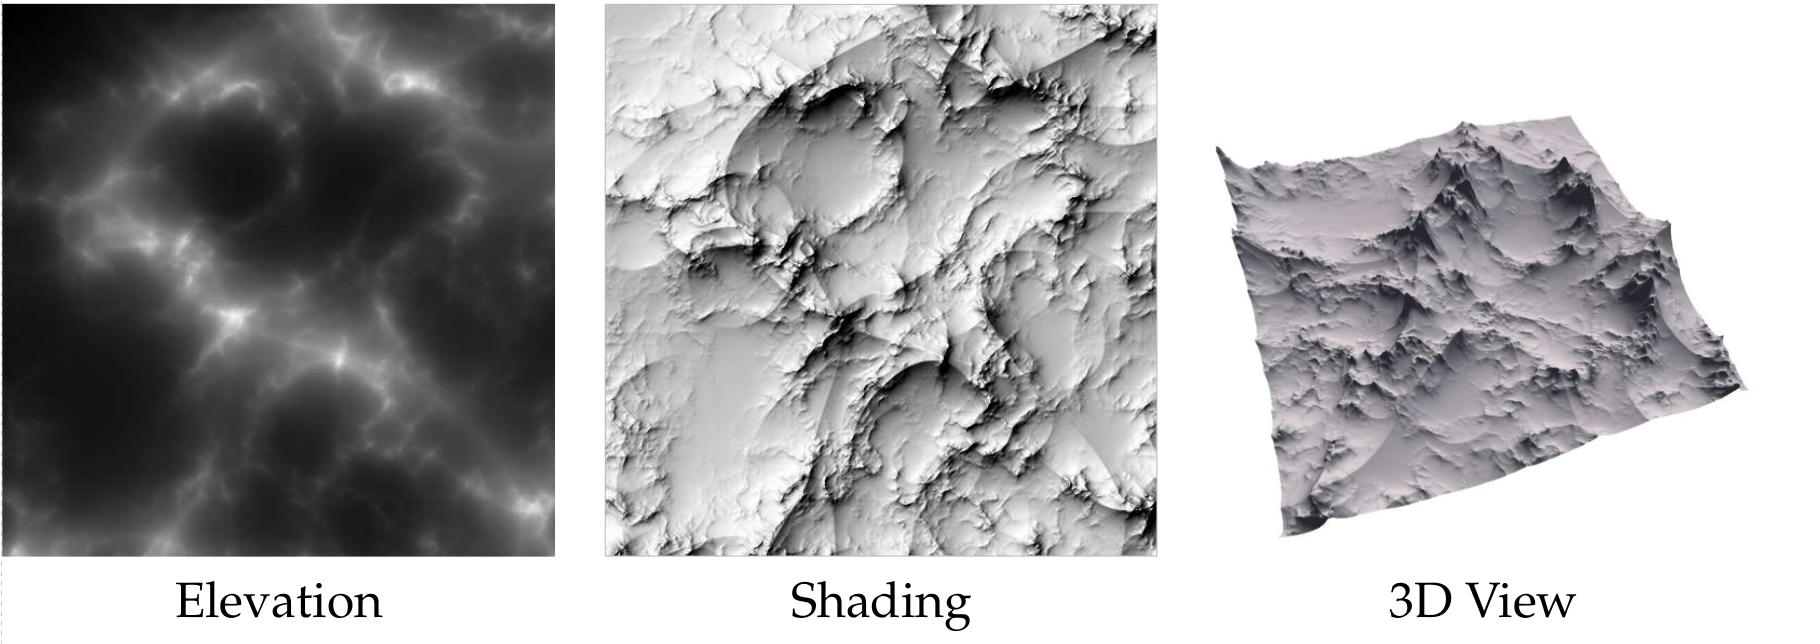
\includegraphics[width=0.75\textwidth]{figuras/hmap.png}
    \caption{Diferentes maneiras de usar um mapa de altura por \cite{dachsbacher2006interactive}}
    \label{fig:hmap}
\end{figure}

Neste trabalho será implementado um sistema de navegação por câmera, oferecendo \textit{3D view}, 
uma visão com perspectiva, isso será útil para visualizar os resultados em diferentes
ângulos, e movimentação sobre o terreno gerado.

\section{Interpolação Linear}

Para a fronteira entre biomas não ser descontinua, mas sim suave, é usado uma interpolação linear entre dois pontos.
Tendo um $x_{0} \leq x \leq x_{1}$, é possível determinar um valor de $y$, baseado em $y_{0}, y_{1}$ usando a distância
de $x$ com $x_{0}$ como peso, representado na equação \ref{eq:interLinear}.

\begin{equation}\label{eq:interLinear}
  \begin{split}
    y = y_{0} + (y_{1} - y_{0}) \cdot \frac{x - x_{0}}{x_{1} - x_{0}}
  \end{split}
\end{equation}

Neste trabalho é usada interpolação linear para suavizar altura e cor quando
o vértice está em área de fronteira. No trabalho de Carli \cite{carli2012canion}, a interpolação 
foi usada para gerar altura entre planaltos de alturas distintas em seus cânyons. No 
trabalho de Bevilacqua \cite{fernando2009costas} foi usada interpolação para definir a textura 
em  determinadas altitudes do terreno.

A função de interpolação usada é a $mix$(mistura). Ela usa o peso de proporção $a$, 
com $a \in \mathbb{Q}: 0 \leq a \leq 1$, para interpolar valores $x$ e $y$. Os valores $x$ e $y$
podem ser uma estrutura de $array$ ou um escalar em $\mathbb{Q}$, mas $x$ e $y$ precisam ser do mesmo tipo.
Essa função está descrita na equação \ref{eq:mixfunc}.

\begin{equation}\label{eq:mixfunc}
  \begin{split}
    mix(x, y, a) = x \cdot (1 - a) + y \cdot a
  \end{split}
\end{equation}

%trabalhos correlatos
%gerador de costas do fenando
%voronoi do indiano
\section{Trabalhos Correlatos}
\subsection{Trabalho de Carli}
O algoritmo para criar o terreno é implementado conforme as
características do bioma alvo, como exemplo, a implementação de Souza
\cite{gabrielle2016canion} e Carli \cite{carli2012canion}, ambos geram relevos de
cânions, como podemos visualizar na figura \ref{fig:carli2012result}.
\begin{figure}[H]
    \centering
    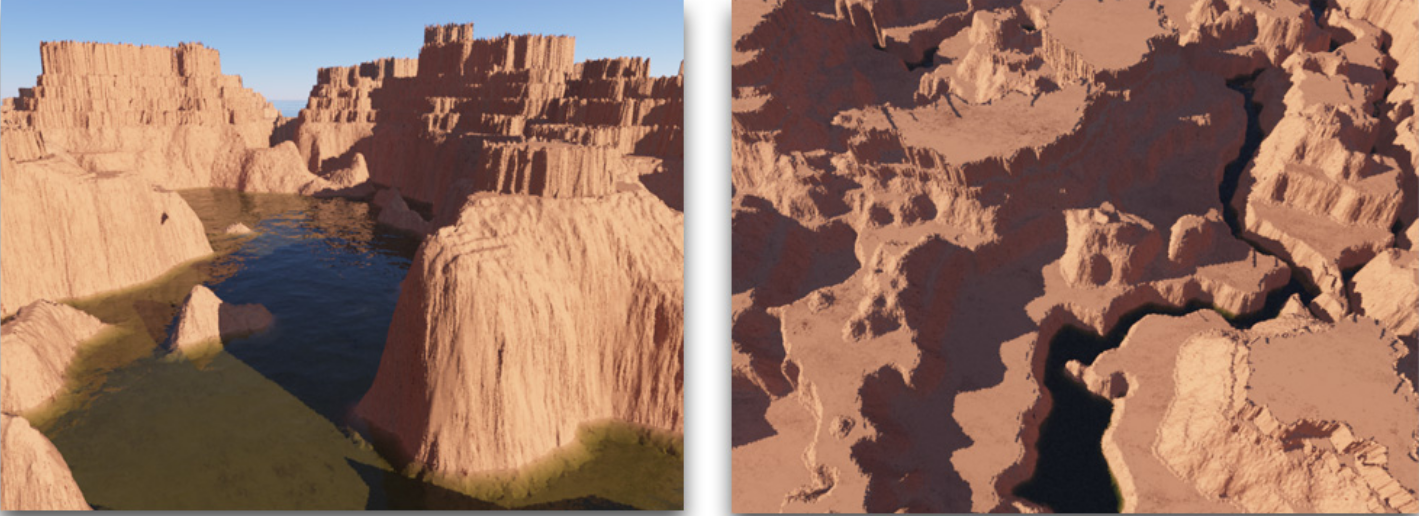
\includegraphics[width=0.9\textwidth]{figuras/carli2012result.png}
    \caption{Resultado do trabalho de \cite{carli2012canion}}
    \label{fig:carli2012result}
\end{figure}

O trabalho do Carli \cite{carli2012canion} não só gera o mapa de altura, mas também
faz busca de percursos de rio e agentes no mapa.

A semelhança do 
trabalho dele com este, é que se faz uso da manipulação dos resultados do ruído
de Perlin para recriar alguns padrões de relevo e também é uma técnica não assistida.


Entretanto, no trabalho  
que apresento aqui, se faz necessário ter pelo menos duas manipulações de ruído distintas
e criar fronteiras contínuas quando as mesmas se encontram. O trabalho 
do Carli \cite{carli2012canion} se preocupa com os parâmetros usados no ruído e manipulação do
resultado, já que o objetivo dele foi criar cânyons realistas. Aqui estes parâmetros serão arbitrários
sem a intensão de criar terrenos realistas, mas sim propor uma técnica que cria terreno de múltiplos biomas com fronteira suaves.

\subsection{Técnica de Patel}
Na técnica de Patel \cite{patel2010polygonal}, que gera ilhas proceduralmente, cada uma podendo ter
múltiplos biomas. Para começar é criado um diagrama de Voronoi, onde cada \textit{site}
vai representar uma região do mapa, os \textit{sites} são gerados em posições
aleatórias, seguido pelo algoritmo de Lloyd's sobre o diagrama para
deixar as regiões mais relaxadas.
Então é usados uma sequencia de ruídos bidimensionais sobre o mapa para decidir
áreas de oceano ou ilha, altura da região e bioma da região, seguido por funções
de ruídos unidimensionais para as bordas da ilha e fronteiras das regiões ter
uma aparência mais natural. O resultado final é ilustrado na
figura \ref{fig:voronoi-map-goal-distorted}.
\begin{figure}[H]
    \centering
    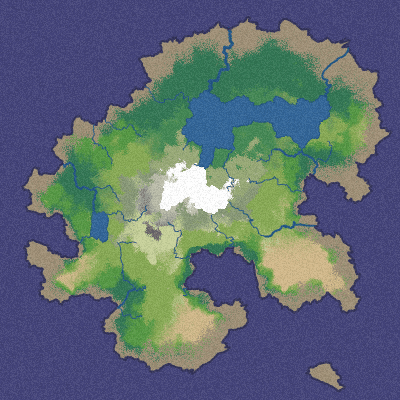
\includegraphics[width=0.4\textwidth]{figuras/voronoi-map-goal-distorted.png}
    \caption{Resultado final de \cite{patel2010polygonal}}
    \label{fig:voronoi-map-goal-distorted}
\end{figure}

Da mesma maneira que Patel \cite{patel2010polygonal} separa zonas e regiões para bioma,
também foi feito neste trabalho, separando o terreno em regiões e 
atribuindo um bioma para cada região. Todavia na técnica mostrada por Patel \cite{patel2010polygonal}
tem regiões demarcadas por um diagrama de Voronoi, enquanto a técnica deste trabalho vai 
usar regiões quadradas de $b$ por $b$ para demarcar áreas de biomas.
A atribuição de um bioma a uma região é feito da mesma maneira que Patel \cite{patel2010polygonal}
usando um identificador da região como entrada para uma função de ruído, em seguida
usando a resposta do ruído para escolher o bioma de determinada região.

O trabalho de Patel \cite{patel2010polygonal} não tem diferentes manipulações de ruído
para biomas distintos, logo todos os biomas tem o mesmo padrão de relevo e as 
fronteiras são contínuas sem necessidade de interpolar fronteiras, que é o 
oposto deste trabalho. Neste trabalho biomas tem características de relevo distintas 
e foi necessário suavizar as fronteiras para mantelas contínuas.

\subsection{Trabalho de Bevilacqua}
O trabalho de Bevilacqua \cite{fernando2009costas} que gera bordas para terrenos, diferente dos 
outros trabalhos correlatos, os terrenos são gerados com tamanhos
pseudo-infinitos, calculando aspectos apenas do terreno perto do jogador ou câmera.

Um dos problemas encontrados por Bevilacqua foi de descontinuidade %foto aqui
nas costas, figura \ref{fig:fe_fe1}. Ele resolveu o problema aplicando ruído unidimensional na distância da costa
para o mar, figura \ref{fig:fe_fe2}. A descontinuidade entre biomas neste trabalho foi resolvida por interpolação 
entre biomas distintos.

\begin{figure}[H]
     \centering
     \subfloat[][]{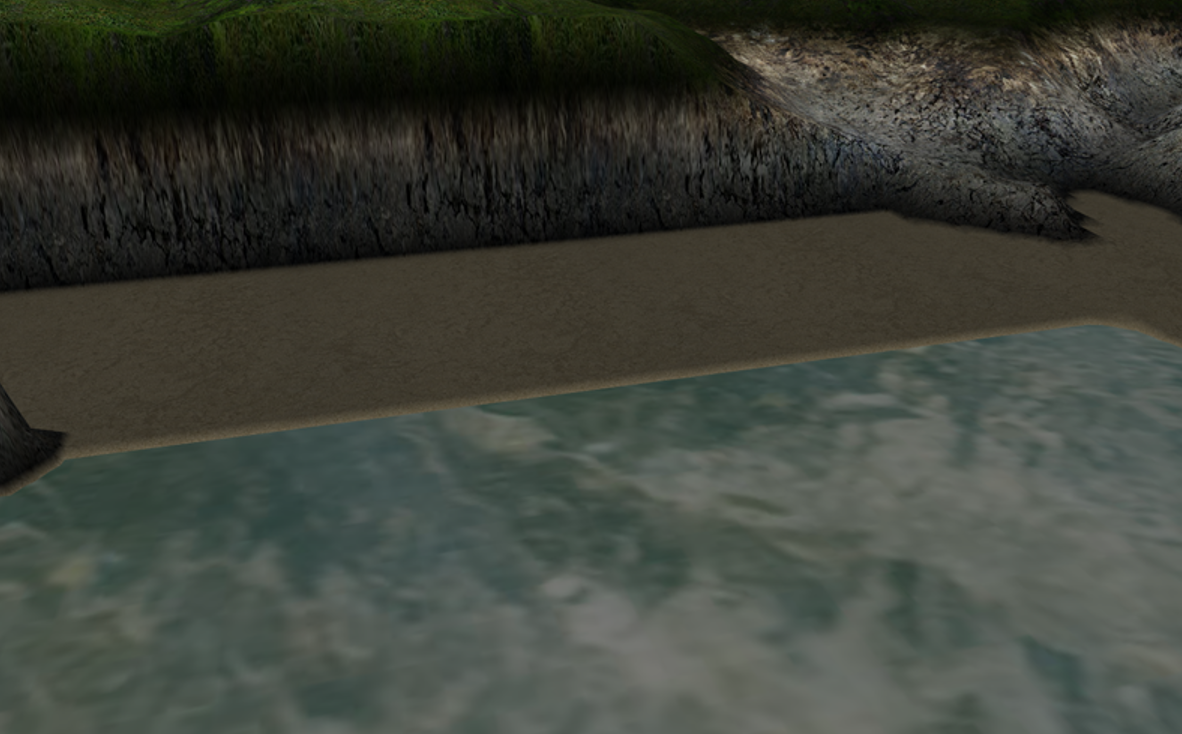
\includegraphics[width=0.45\textwidth]{figuras/fe/fe1.png}\label{fig:fe_fe1}}\hspace{0.1cm}
     \subfloat[][]{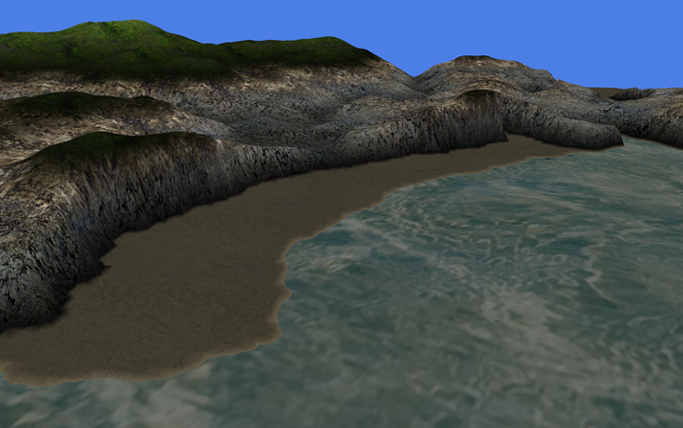
\includegraphics[width=0.45\textwidth]{figuras/fe/fe2.png}\label{fig:fe_fe2}}
     \caption{Amostras do trabalho de \cite{fernando2009costas}.}
     \label{fig:fefefefefe}
     % usar \hspace{0.1cm}, é gambiarra mas funciona
\end{figure}